../cictikz/src/cictikz/data/tex/cictikz_preamble.tex

% Drain current against drain voltage at a fixed gate voltage.
%
% The steep part on the left is the triode region, where the device is a
% voltage controlled resistor. Past roughly 0.2 V it saturates and the
% current stops caring much about the drain.
%
% "Stops caring much" is the useful part. The curve is not flat, it keeps
% a small slope, and that slope is the output conductance that limits the
% gain of every amplifier in this course.
%
% Generated by py/tikzplot.py. Edit the script in ex/ that
% produced it and re-run that, not this file.

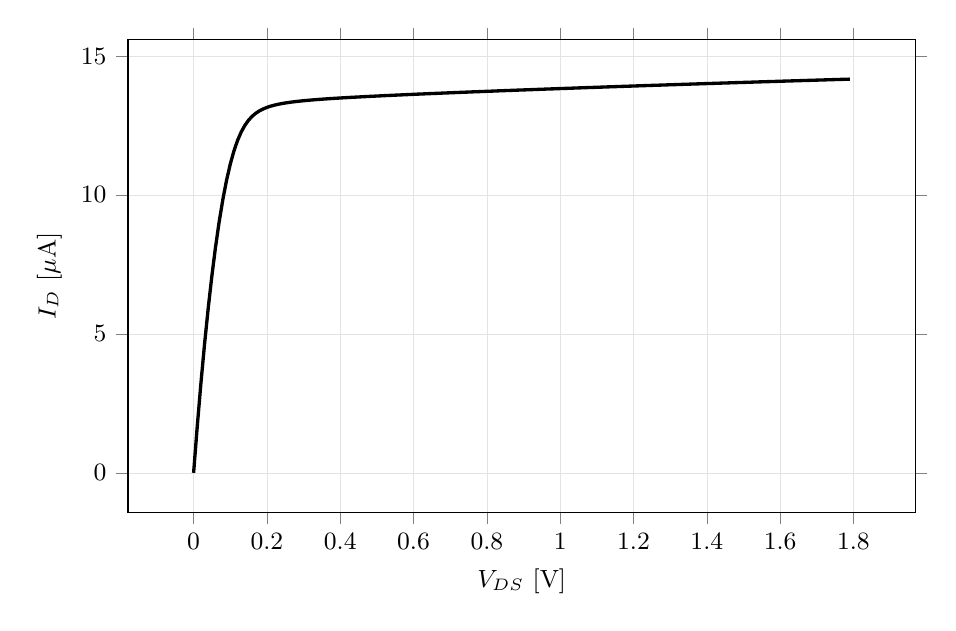
\begin{tikzpicture}[thick]

\begin{axis}[
  width=10.0cm,
  height=6.0cm,
  scale only axis,
  grid=both,
  grid style={gray!22, very thin},
  tick align=outside,
  tick label style={font=\small},
  label style={font=\small},
  title style={font=\small, yshift=-1mm},
  legend cell align=left,
  legend style={font=\small, draw=gray!50, fill=white, fill opacity=0.85, text opacity=1},
  xlabel={$V_{DS}$ [V]},
  ylabel={$I_D$ [$\mu$A]}
]
\addplot[black, very thick, mark=none] coordinates {(0,3.5903e-05) (0.01,1.6836) (0.02,3.2346) (0.03,4.6544) (0.04,5.9446) (0.05,7.1071) (0.06,8.1441) (0.07,9.0586) (0.08,9.8542) (0.09,10.536) (0.1,11.109) (0.11,11.582) (0.12,11.966) (0.13,12.27) (0.14,12.508) (0.15,12.692) (0.16,12.834) (0.17,12.944) (0.18,13.029) (0.19,13.096) (0.2,13.15) (0.21,13.194) (0.22,13.23) (0.23,13.26) (0.24,13.287) (0.25,13.309) (0.26,13.329) (0.27,13.347) (0.28,13.363) (0.29,13.377) (0.3,13.391) (0.31,13.403) (0.32,13.415) (0.33,13.426) (0.34,13.436) (0.35,13.446) (0.36,13.455) (0.37,13.464) (0.38,13.473) (0.39,13.481) (0.4,13.489) (0.41,13.497) (0.42,13.505) (0.43,13.512) (0.44,13.519) (0.45,13.526) (0.46,13.533) (0.47,13.54) (0.48,13.547) (0.49,13.553) (0.5,13.56) (0.51,13.566) (0.52,13.573) (0.53,13.579) (0.54,13.585) (0.55,13.591) (0.56,13.597) (0.57,13.603) (0.58,13.609) (0.59,13.615) (0.6,13.621) (0.61,13.627) (0.62,13.632) (0.63,13.638) (0.64,13.644) (0.65,13.649) (0.66,13.655) (0.67,13.66) (0.68,13.666) (0.69,13.671) (0.7,13.677) (0.71,13.682) (0.72,13.687) (0.73,13.693) (0.74,13.698) (0.75,13.703) (0.76,13.709) (0.77,13.714) (0.78,13.719) (0.79,13.724) (0.8,13.729) (0.81,13.734) (0.82,13.739) (0.83,13.745) (0.84,13.75) (0.85,13.755) (0.86,13.76) (0.87,13.765) (0.88,13.77) (0.89,13.775) (0.9,13.78) (0.91,13.784) (0.92,13.789) (0.93,13.794) (0.94,13.799) (0.95,13.804) (0.96,13.809) (0.97,13.814) (0.98,13.818) (0.99,13.823) (1,13.828) (1.01,13.833) (1.02,13.837) (1.03,13.842) (1.04,13.847) (1.05,13.852) (1.06,13.856) (1.07,13.861) (1.08,13.866) (1.09,13.87) (1.1,13.875) (1.11,13.879) (1.12,13.884) (1.13,13.889) (1.14,13.893) (1.15,13.898) (1.16,13.902) (1.17,13.907) (1.18,13.911) (1.19,13.916) (1.2,13.92) (1.21,13.925) (1.22,13.929) (1.23,13.934) (1.24,13.938) (1.25,13.943) (1.26,13.947) (1.27,13.951) (1.28,13.956) (1.29,13.96) (1.3,13.965) (1.31,13.969) (1.32,13.973) (1.33,13.978) (1.34,13.982) (1.35,13.986) (1.36,13.991) (1.37,13.995) (1.38,13.999) (1.39,14.004) (1.4,14.008) (1.41,14.012) (1.42,14.016) (1.43,14.021) (1.44,14.025) (1.45,14.029) (1.46,14.033) (1.47,14.038) (1.48,14.042) (1.49,14.046) (1.5,14.05) (1.51,14.054) (1.52,14.058) (1.53,14.063) (1.54,14.067) (1.55,14.071) (1.56,14.075) (1.57,14.079) (1.58,14.083) (1.59,14.087) (1.6,14.091) (1.61,14.096) (1.62,14.1) (1.63,14.104) (1.64,14.108) (1.65,14.112) (1.66,14.116) (1.67,14.12) (1.68,14.124) (1.69,14.128) (1.7,14.132) (1.71,14.136) (1.72,14.14) (1.73,14.144) (1.74,14.148) (1.75,14.152) (1.76,14.156) (1.77,14.16) (1.78,14.164) (1.79,14.168)};
\end{axis}

\end{tikzpicture}
\end{document}
